\chapter{图像的插入示例}
\label{cha:fig_example}
除了第一章引言和最后一章的总结与展望之外,正文的所有章都要在章标题之下加上这样一段引入本章内容的话语,让读者知道本章的目的以及意义。本章将通过一些示例来说明如何插入图片。读者在阅读文章时,最能吸引读者注意力的莫过于文章中的图片,因此图片对于论文来说是重中之重,甚至可以说,好图就是好文章。规范地插入图片对于整篇文章的观感、阅读体验来说,有着至关重要的作用。
\section{单张图片的插入}
\label{sec:fig_singlefig}
单张图片插入的原则:(1)图片居中放置,大小适当,图中文字、内容清晰;(2)从文献中获得的图片要引用,要写明来源;(3)图片应该放置在两段文字之间,图片上面一段文字应该是对图片内容的描述,不要插在一段文字内,一页排不下时,应排在下一页的顶部;(4)对图片的描述要符合规范,指明是图x-x,不能说如下图所示。
\begin{itemize}
\item 错误描述:托卡马克装置示意图如下图所示\cite{xu2016general}:
\item 正确描述:托卡马克装置示意图如图 \ref{fig:tokamak} 所示\cite{xu2016general}:
\end{itemize}

\begin{figure}[htbp] % 图片排序优先级,h表示当前位置,t表示顶部,b表示底部,p表示浮动页,可以是单独一个字母或者几个字母的组合
	% 居中
	\centering
	% 图片宽度、图片文件名及在硬盘中的位置
	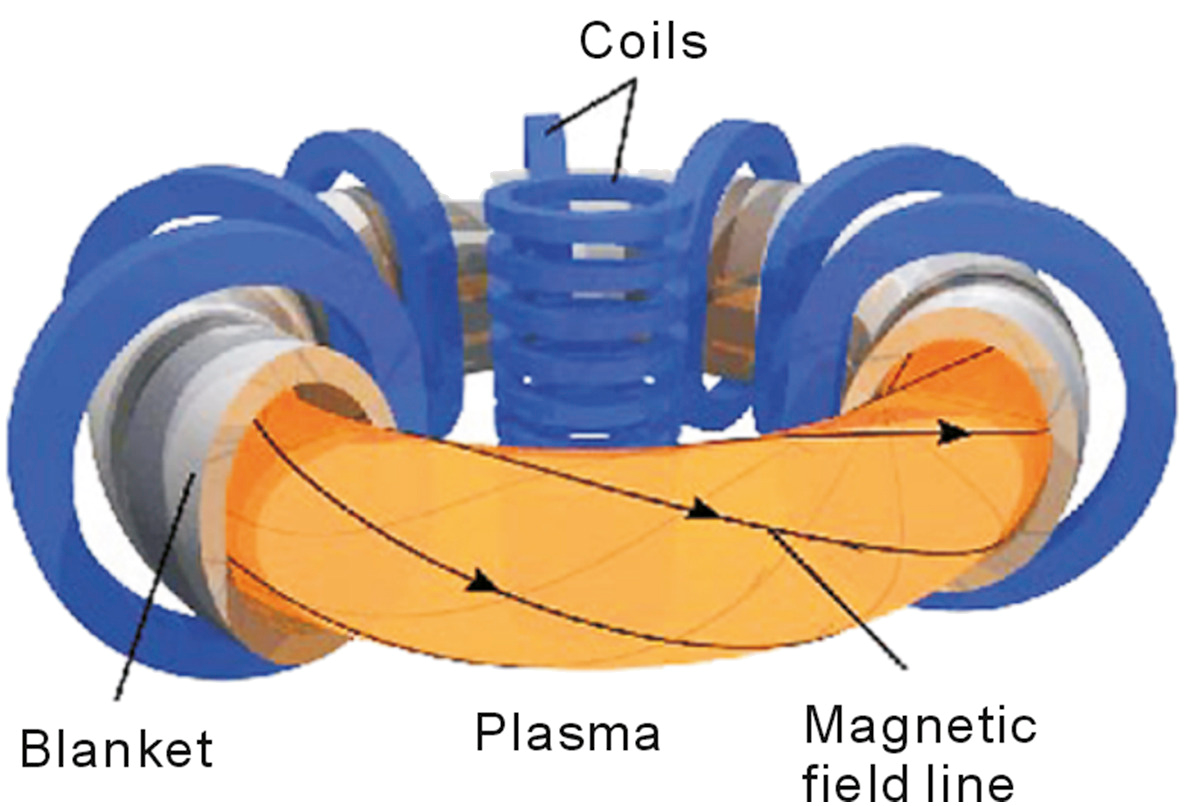
\includegraphics[width=0.6\textwidth]{image/chap03/tokamak.png}
	% 图片下标题
	\caption{托卡马克装置示意图\cite{xu2016general}}
	% 图片标签
	\label{fig:tokamak}
\end{figure}
\subsection{矢量图片的插入}
\label{ssec:fig_vecfig}
本小节示例了如何插入小节。按照中大的规定,正文中的标题只到小节,如 \ref{ssec:fig_vecfig} 小节,目录中的标题只到节,如 \ref{sec:fig_singlefig} 节。

\LaTeX\  中pdf和eps格式的矢量图是能直接插入的,操作很简单,与插入图 \ref{fig:tokamak} 的操作相同,只需更改文件名。

\section{多张图片的插入}
\label{sec:fig_multifig}
多张图片插入的原则与单张图片的相同,但是值得注意的是,多张图片不宜使用\LaTeX\ 直接插入,应将所需插入的图片先用PowerPoint排列、拼接,再标号,生成一张图片,再整个插入论文中,这样就与单张图片的插入过程相同。生成图片的过程,偷懒的话可以直接截屏保存为png格式图片,不偷懒就调整ppt的大小后直接导出为pdf。

